\documentclass[xcolor=dvipsnames]{beamer}

% Copyright 2010 by Brendan W. McAdams <brendan@10gen.com>
%
% You may redistribute the content of this presentation for your own needs 
% provided you give credit to its author. In other words: "Don't be a dick."
% % Latex code based upon the "Generic Presentation 15-45 minutes" template from Beamer.

\mode<presentation>
{
  % \usetheme{Dresden}      
  \usetheme{Madrid}
  \setbeamercolor{structure}{fg=OliveGreen!125!black} 
        
  % \usecolortheme{dolphin}
  \setbeamercovered{transparent}
}


\usepackage{hyperref}
\usepackage{xcolor}
\usepackage{listings}

\hypersetup{backref,  
pdfpagemode=FullScreen,  
colorlinks=false}

 % "define" Scala
\lstdefinelanguage{Scala}{
   morekeywords={abstract,case,catch,class,def,%
     do,else,extends,false,final,finally,%
     for,forSome,if,implicit,import,lazy,%
     match,mixin,%
     new,null,object,override,package,%
     private,protected,requires,return,sealed,%
     super,this,throw,trait,true,try,%
     type,val,var,while,with,yield},
   otherkeywords={=>,<-,<\%,<:,>:,\#,@},
   sensitive=true,
   morecomment=[l]{//},
   morecomment=[n]{/*}{*/},
   morestring=[b]",
   morestring=[b]',
   morestring=[b]"""
 }


\lstdefinelanguage{JavaScript}{
    keywords={typeof, new, true, false, catch, function, return, null, catch, switch, var, if, in, while, do, else, case, break}
    keywordstyle=\color{blue}\bfseries,
    ndkeywords={class, export, boolean, throw, implements, import, this},
    ndkeywordstyle=\color{darkgray}\bfseries,
    identifierstyle=\color{black},
    sensitive=false,
    comment=[l]{//},
    morecomment=[s]{/*}{*/},
    commentstyle=\color{purple}\ttfamily,
    stringstyle=\color{red}\ttfamily,
    morestring=[b]',
    morestring=[b]"
}
\usepackage{caption}
\DeclareCaptionFont{white}{\color{white}}
\DeclareCaptionFormat{listing}{\colorbox{black}{\parbox{\textwidth}{#1#2#3}}}
\captionsetup[lstlisting]{format=listing,labelfont=white,textfont=white}


\usepackage{color}
\definecolor{dkgreen}{rgb}{0,0.6,0}
\definecolor{gray}{rgb}{0.5,0.5,0.5}
\definecolor{mauve}{rgb}{0.58,0,0.82}
\definecolor{lightgray}{rgb}{.9,.9,.9}
\definecolor{darkgray}{rgb}{.4,.4,.4}
\definecolor{purple}{rgb}{0.65, 0.12, 0.82}

% Default settings for code listings
\lstset{
  frame=tb,%
  language=Scala,%
  aboveskip=1.5mm,%
  belowskip=1.5mm,%
  xleftmargin=1mm,%
  xrightmargin=1mm,%
  showstringspaces=false,%
  keepspaces=true,%
  columns=[c]fixed,%
  basicstyle={\tiny\ttfamily},%
  escapechar=¤,%
  numbers=none,%
  numberstyle=\tiny\color{yellow},%
  keywordstyle=\color{blue},%
  commentstyle=\color{dkgreen},%
  stringstyle=\color{mauve},%
  frame=single,%
  breaklines=true,%
  breakatwhitespace=true,%
  tabsize=4,%
  firstnumber=0,%
  numbersep=1.5mm,%
  numberstyle=\tiny%
}

% \lstdefinestyle{floating}{%
%     xleftmargin=10pt,%
%     xrightmargin=5pt,%
%     aboveskip=4mm,%
%     belowskip=4mm,%
%     fontadjust=true,%
%     columns=[c]flexible,%
%     keepspaces=true,%
%     basewidth={0.5em, 0.425em},%
%     tabsize=2,%
%     basicstyle=\renewcommand{\baselinestretch}{0.95}\ttfamily,%
%     commentstyle=\rm,%
%     keywordstyle=\bfseries,%
%     mathescape=true,%
%     captionpos=b,%
%     framerule=0.3pt,%
%     firstnumber=0,%
%     numbersep=1.5mm,%
%     numberstyle=\tiny,%
%     float=tbp,%
%     frame=tblr,%
%     framesep=5pt,%
%     framexleftmargin=3pt,%
%     abovecaptionskip=\smallskipamount,%
%     belowcaptionskip=\smallskipamount,%
% } % to define: caption, label

\newcommand{\code}[1]{%
    \lstinline[%keywordstyle=,%
               flexiblecolumns=true,%
               basicstyle=\ttfamily]_#1_}

\newenvironment{itemizeframe}
               {\begin{frame}\startitemizeframe} 
               {\stopitemizeframe\end{frame}}
              
\newenvironment{codeframe}
                {\begin{frame}[allowframebreaks,allowdisplaybreaks]}
                {\end{frame}}
                
\newenvironment{itemizecodeframe}
              {\begin{frame}[allowframebreaks,allowdisplaybreaks]
              \startitemizeframe} 
              {\stopitemizeframe\end{frame}}

\newcommand\startitemizeframe{\begin{itemize}} \newcommand\stopitemizeframe{\end{itemize}}

\usepackage[english]{babel}
% or whatever

\usepackage[latin1]{inputenc}
% or whatever

\usepackage{times}
\usepackage[T1]{fontenc}
% Or whatever. Note that the encoding and the font should match. If T1
% does not look nice, try deleting the line with the fontenc.


\title{WTF Is An Implicit?!?} % (optional, use only with long paper titles)

\institute[10gen, Inc.]{10gen, Inc.}

%\subtitle
%{Presentation Subtitle} % (optional)

\author[B.W. McAdams]{Brendan W. McAdams}
% - Use the \inst{?} command only if the authors have different
%   affiliation.

\date{NY Scala Enthusiasts}

\subject{Scala Implicits}
% This is only inserted into the PDF information catalog. Can be left
% out. 


\logo{
\includegraphics[width=2.25cm]{images/mongodb-logo}}


% Delete this, if you do not want the table of contents to pop up at
% the beginning of each subsection:
% \AtBeginSubsection[]
% {
%   \begin{frame}<beamer>
%   \frametitle{Outline}
%     \tableofcontents[currentsection,currentsubsection,currentsubsubsection]
%   \end{frame}
% }


% If you wish to uncover everything in a step-wise fashion, uncomment
% the following command: 

% \beamerdefaultoverlayspecification{<+->}


\begin{document}

\begin{frame}
  \titlepage
\end{frame}

\section{Scala Implicits}

\begin{itemizeframe}
    \frametitle{Types of Implicits}
    \framesubtitle{Major Coverages}
    \item Implicit Parameters
    \item Implicit Methods
    \item Pimp My Library
    \item Type Classes
\end{itemizeframe}

\subsection{Implicit Parameters}
\begin{itemizeframe}
    \frametitle{Implicit Parameters}
    \framesubtitle{What Are Implicit Parameters?}
    \item `Explicit' parameter indicates a method argument you pass, well \emph{explicitly}.
    \item `Implicit' indicates a method argument which is\ldots \emph{implied}. (But you can pass them explicitly too!)
    \item The value of an implicit argument is inferred from the scope by default; it can be used to define an environmental context.
    \item Useful for:
        \begin{itemize}
            \item Values which are initialized once in scope and you don't want to keep passing explicitly.
            \item Passing utility libraries such as conversion methods to conform to a protocol.
        \end{itemize}
\end{itemizeframe}

\begin{itemizeframe}
    \frametitle{Implicit Parameters}
    \framesubtitle{Demonstrated\ldots}
    \item Implicit parameters are passed as an additional argument list:
        \lstinputlisting{code/implicit_sample_arg1.scala}
    \pause
    \item How does this differ from default arguments? 
\end{itemizeframe}

\subsection{Caveats}
\begin{itemizeframe}
    \frametitle{Caveats of Implicits}
    \item Caveat \#1: Scala will {\em not} try to second guess you with ambiguity.  It {\em will} fail to compile.
        \lstinputlisting{code/implicit_ambiguity.scala}
        
\end{itemizeframe}

\subsection{Implicit Conversions}
\begin{frame}
    \frametitle{Fitting A Square Peg Into a Round Hole}
        In Strongly Typed languages (e.g. Java), square pegs do {\em not} fit into round holes:
        \begin{center}
        
\includegraphics{images/square-peg-round-hole.jpg}
        \end{center}
\end{frame}
\begin{frame}
    \frametitle{Fitting A Square Peg Into a Round Hole}
        In Loosely Typed languages (e.g. Perl), round holes can be convinced to accept square pegs:
        \begin{center}
        
\includegraphics[scale=0.25]{images/rabbitduck4.jpg}
        \end{center}
\end{frame}

\begin{frame}
    \frametitle{Fitting A Square Peg Into a Round Hole}
        With Scala, you get a lathe instead:
        \begin{center}
        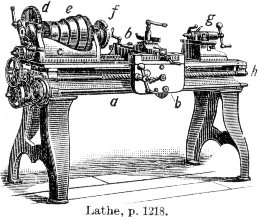
\includegraphics[scale=0.5]{images/Lathe.png}
        \end{center}
\end{frame}

\begin{itemizecodeframe}
    \frametitle{Implicit Conversions}
    \item You can declare {\em methods} to be implicit as well as {\em values}
    \item When Scala's compiler encounters an invalid argument type being passed to a method:
        \lstinputlisting{code/implicit_sample_method1.scala}
    \pagebreak
    \item If it finds a matching implicit method (takes bad type and returns good type) in scope, and no ambiguity\ldots Square Pegs can become Round Pegs:
        \lstinputlisting{code/implicit_sample_method2.scala}
    \item In a dynamic language, this may be called ``monkey patching''. Unlike Perl, Python, etc. Scala resolves implicits at compile time.
\end{itemizecodeframe}

\subsection{Caveats}
\begin{itemizeframe}
    \frametitle{Caveats of Implicits}
    \item Caveat \#2: Normal Type Boundaries \code{ def foo[A <: SomeComplexType] } will {\em not} allow implicit conversions.  
    \item Use View Boundaries \code { def foo[A <\% SomeComplexType] } instead!
\end{itemizeframe}

\section{Implicit Tricks}
\begin{itemizeframe}
    \frametitle{Tricks with Implicits}
    \item Scala's Compiler lets you use Implicits to pull off a few tricks\ldots
\end{itemizeframe}

\subsection{Pimp My Library}
\begin{frame}
    \frametitle{Pimpin' Your Library}
    \begin{center}
    
\includegraphics[scale=0.5]{images/players_ball_southpark-600x335.png}
    \end{center}
\end{frame}
\begin{itemizeframe}
    \frametitle{Pimpin' Your Library}
    \item Implicit methods allow for the the ``Pimp My Library Pattern''
    \item Coined by Martin Odersky in a 2006 Blog post.  Similar to C\# extension methods, Ruby modules.
    \item Uses implicit conversions to tack on new methods at runtime.
    \item Either return a new ``Rich\_'' or anonymous class\ldots
        \lstinputlisting{code/pimp_sample1.scala}
\end{itemizeframe}

\subsection{Type Classes}
\begin{itemizecodeframe}
    \frametitle{Type Classes}
    \item Finally, Implicit parameters allow for emulating Type Classes
    \item Lets you create a list of ``Acceptable'' divergent values which can pass a single type boundary
    \item Used heavily in Scala 2.8 for constructs such as Numeric, Ordering and CanBuildFrom
    \pagebreak
    \item A Vending Machine could accept divergent funding:
        \lstinputlisting{code/type_classes.scala}
    \item No real leeway, must explicitly define {\bf all} acceptable classes, won't pass a subclass of a declared type
    \item Use scala.math.Numeric with this boundary trick to accept any numeric type (Double, Int, Float, BigDecimal, Short, etc etc)
    \item Type Classes described in great detail by D.C. Sobral at \url{http://dcsobral.blogspot.com/2010/06/implicit-tricks-type-class-pattern.html}
    \pagebreak
    \item Bonus Feature: Variant of the Type Class boundary syntax lets you capture manifests in 2.8.x:
        \lstinputlisting{code/manifest_fu.scala}
\end{itemizecodeframe}

\begin{itemizeframe}
    \frametitle{Questions?}
    \framesubtitle{Contact Info}
        \item twitter: {\bf @rit}
        \item email: {\bf brendan@10gen.com}	
		\item {\Large 10gen is {\em hiring!}  We need smart engineers in both NY and Bay Area: \url{http://10gen.com/jobs}}
\end{itemizeframe}



\end{document}
